\chapter{Viscous Plane Flows}
\label{chap:viscousplane}
This report is focused on \emph{viscous plane flows}. A plane flow is a 2 dimensional flow represented by a velocity profile $ U $ in a single direction. For this project, we will consider $ U $ that are functions of $ z $ only and act in the $ x $ direction. Moreover, our flow will be bounded between $ z = z_{1_*} $ and $ z = z_{1_*} $. Figure \ref{fig:pflow} shows the system we will be analysing in an initial stable state. 

\begin{figure}[htb!]
    \centering
    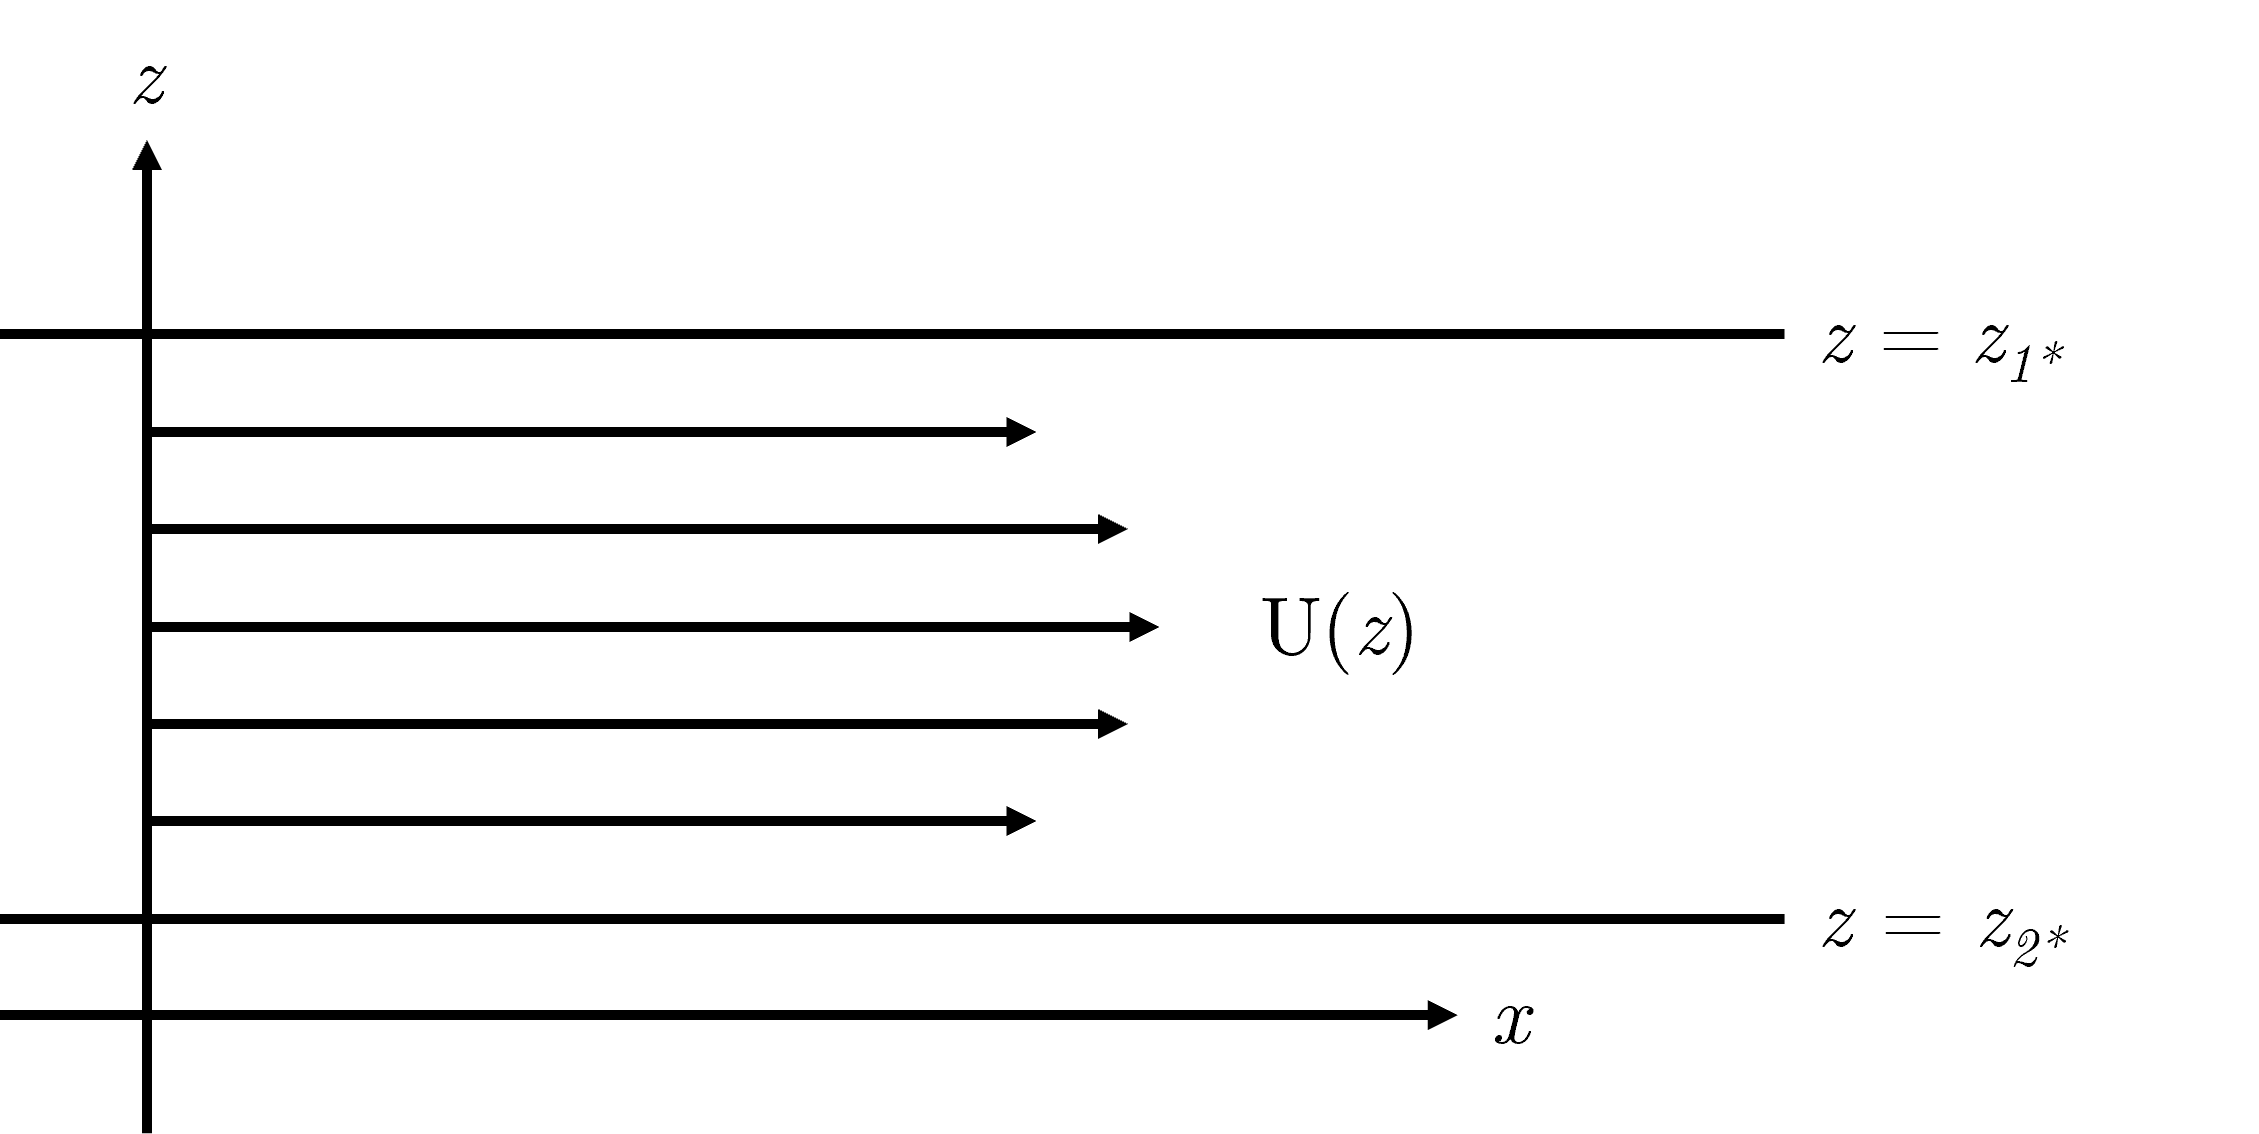
\includegraphics[width=10cm]{figures/PSF.png}
    \caption{The setup of our flow}
    \label{fig:pflow}
\end{figure}

\section{Basic state and governing equations}
\textbf{check the notation used for the dimensional v dimensionless cases, make sure it is consistent}

The fluid discussed in this report is considered to have a constant density i.e. $ \rho = \text{const.} $

Let us use the basic steady flow as defined in \citet{drazin2004hydrodynamic} with the form
\begin{equation}
    \mathbf{U}_* = U_* (z_*) \mathbf{i} \hspace{10px} (z_{1_*} \leq z_* \leq z_{2_*}),
\end{equation}
and boundaries on $z_* = z_{1_*} \text{and } z_{2_*}$ that are either \emph{rigid} or \emph{free}:
\begin{itemize}
    \item \emph{rigid} - normal component of velocity must vanish
    \item \emph{free} - pressure must be constant
\end{itemize}

For this flow, we have the following governing equations that must be satisfied:
\begin{align}
    \div{\mathbf{u_*}} &= 0, \nonumber\\
    \pdv{\mathbf{u_*}}{t_*} + \mathbf{u_*} \cdot \nabla \mathbf{u_*} &= - \frac{1}{\rho} \nabla p_* + \nu \Delta \mathbf{u_*}.
\label{dimgoveq}
\end{align}
These equations are the continuity equation and Navier-Stokes equation for an incompressible fluid respectively. Note that we denote the \emph{kinematic viscosity} $ \nu = \frac{\mu}{\rho} $ and have also set $ f = 0 $ in the Navier-Stokes equation, assuming there is no force acting on the fluid.

\section{Deriving the dimensionless form of our governing equations}
To write the governing equations in terms of dimensionless quantities we utilise the following change of variables. We begin by defining
\begin{align}
    V &= \text{max}_{z_* \in [z_{1_*}, z_{2_*}]} |U_* (z_*)|, \nonumber\\
    L &= \frac{1}{2}(z_{2_*} - z_{1_*})
\end{align}
We will refer to $ V $ as the \emph{characteristic velocity} and $ L $ as the \emph{characteristic length}. Now change our other variables to their dimensionless forms
\begin{align}
    t = \frac{t_* V}{L},\ \mathbf{x} &= \frac{\mathbf{x_*}}{L},\ \mathbf{u} = \frac{\mathbf{u_*}}{V},\ p = \frac{p}{\rho V^2}, \nonumber\\ \mathbf{U} &= \frac{\mathbf{U_*}}{V} \equiv U(z) \mathbf{i} 
\end{align}
We can use this transformation to find dimensionless forms of the various derivatives in the governing equations. By the chain rule we have
\begin{equation}
    \pdv{\mathbf{u}}{t} = \pdv{\mathbf{u}}{\mathbf{u_*}} \pdv{\mathbf{u_*}}{t_*} \pdv{t_*}{t} = \frac{L}{V^2} \pdv{\mathbf{u_*}}{t_*} \implies \pdv{\mathbf{u_*}}{t_*} = \frac{V^2}{L} \pdv{\mathbf{u}}{t},
\label{dut*}
\end{equation}
and
\begin{gather}
    (\nabla \mathbf{u_*})^\mu = \pdv{\mathbf{u_*}}{{x_*}^\mu} = \pdv{\mathbf{u_*}}{\mathbf{u}} \pdv{\mathbf{u}}{x^\mu} \pdv{x^\mu}{{x_*}^\mu} = \frac{V}{L} \pdv{\mathbf{u}}{x^\mu} = \frac{V}{L} (\nabla \mathbf{u})^\mu \nonumber\\
    \implies \nabla \mathbf{u_*} = \frac{V}{L} \nabla \mathbf{u}.
\label{gradu*}
\end{gather}

\textbf{the below needs updating i think or some explanation of what is being done here}

Similarly
\begin{gather}
    (\Delta \mathbf{u_*})^\mu) = \pdv{{x_*}^\mu} (\nabla \mathbf{u_*})^\mu = \frac{1}{L} \pdv{x^\mu}(\frac{V}{L} (\nabla \mathbf{u})^\mu) = \frac{V^2}{L} (\Delta \mathbf{u})^\mu \nonumber\\
    \implies \Delta \mathbf{u_*} = \frac{V^2}{L} \Delta \mathbf{u},
\label{lapu*}
\end{gather}
and
\begin{gather}
    \div{\mathbf{u_*}} = \pdv{{u_*}^\mu}{{x_*}^\mu} = \frac{V}{L} \pdv{u^\mu}{x^\mu} = \frac{V}{L} \div{\mathbf{u}}.
\label{divu*}
\end{gather}
Finally, for $ p_* $ we need just $ \nabla p_* $ in terms of $ \nabla p $, again using the chain rule we obtain
\begin{gather}
    (\nabla p_*)^\mu = \pdv{p_*}{{x_*}^\mu} = \pdv{p_*}{p} \pdv{p}{x^\mu} \pdv{x^\mu}{{x_*}^\mu} = \rho V^2 \pdv{p}{x^\mu} \frac{1}{L} = \frac{\rho V^2}{\mu} \pdv{p}{x^\mu} \nonumber\\
    \implies \nabla p_* = \frac{\rho V^2}{L} \nabla 
\label{gradp*}
\end{gather}
We can now substitute these results into our governing equations \eqref{dimgoveq} to get their dimensionless forms. For the \emph{continuity equation} we use equation \eqref{divu*} to get
\begin{gather}
    0 = \div{\mathbf{u_*}} = \frac{V}{L} \div{\mathbf{u}} \implies \div{\mathbf{u}} = 0.
\end{gather}
Substituting our remaining equations \eqref{dut*}, \eqref{gradu*}, \eqref{lapu*}, \eqref{gradp*} into the \emph{Navier-Stokes equation} we get
\begin{align}
        \pdv{\mathbf{u_*}}{t_*} + \mathbf{u_*} \cdot \nabla \mathbf{u_*} &= - \frac{1}{\rho} \nabla p_* + \nu \Delta \mathbf{u_*} \nonumber\\
        \implies \frac{V^2}{L} \pdv{\mathbf{u}}{t} + (V \mathbf{u}) \cdot (\frac{V}{L}\nabla \mathbf{u}) &= - \frac{1}{\rho} (\frac{\rho V^2}{L} \nabla p) + \nu (\frac{V}{L^2} \Delta \mathbf{u}) \nonumber\\
        \implies \frac{V^2}{L} \pdv{\mathbf{u}}{t} + \frac{V^2}{L} \mathbf{u} \cdot \nabla \mathbf{u} &= -\frac{V^2}{L} \nabla p + \frac{\nu V}{L^2} \Delta \mathbf{u} \nonumber\\
        \implies \pdv{\mathbf{u}}{t} + \mathbf{u} \cdot \nabla \mathbf{u} &= -\nabla p + \frac{\nu}{V L} \Delta \mathbf{u}
\end{align}
Notice that $ \frac{V L}{\nu} $ is the famous \emph{Reynold's number} $ R $. Using this in the Navier-Stokes equation leaves us with our pair of \emph{dimensionless governing equations}
\begin{align}
    \div{\mathbf{u}} &= 0, \nonumber\\
    \pdv{\mathbf{u}}{t} + \mathbf{u} \cdot \nabla \mathbf{u} &= -\nabla p + R^{-1} \Delta \mathbf{u}.
\label{dlessgoveq}
\end{align}

Substituting $ \mathbf{u}(\mathbf{x}, t) = U(z) \mathbf{i} $, $ p (\mathbf{x}, t) = $ into \eqref{dlessgoveq}, we find that $ U(z) $ must satisfy the following equation of motion 
\begin{equation}
    \dv[2]{U}{z} = R \dv{P}{x}
\end{equation}
which limits our choices of $ U (z) $. There are two main important cases defined as follows:
\begin{list}{$-$}{\leftmargin=1cm}
    \item \emph{Poiseuille flow}: $ U(z) = 1 - z^2 $ with $ \dv{P}{x} = const. $
    \item \emph{Couette flow}: $ U(z) = z $ with $ P = const. $
\end{list}

Schematic diagrams for these 2 flows can be seen in Figure \ref{fig:pandcflow}. This leaves us with a family of flows to analyse formed by a linear combination of these 2 types of flow.

\textbf{discuss where these may occur in the real world?}

\begin{figure}[htb!]
    \centering
    \subfloat[Poiseuille flow]{
    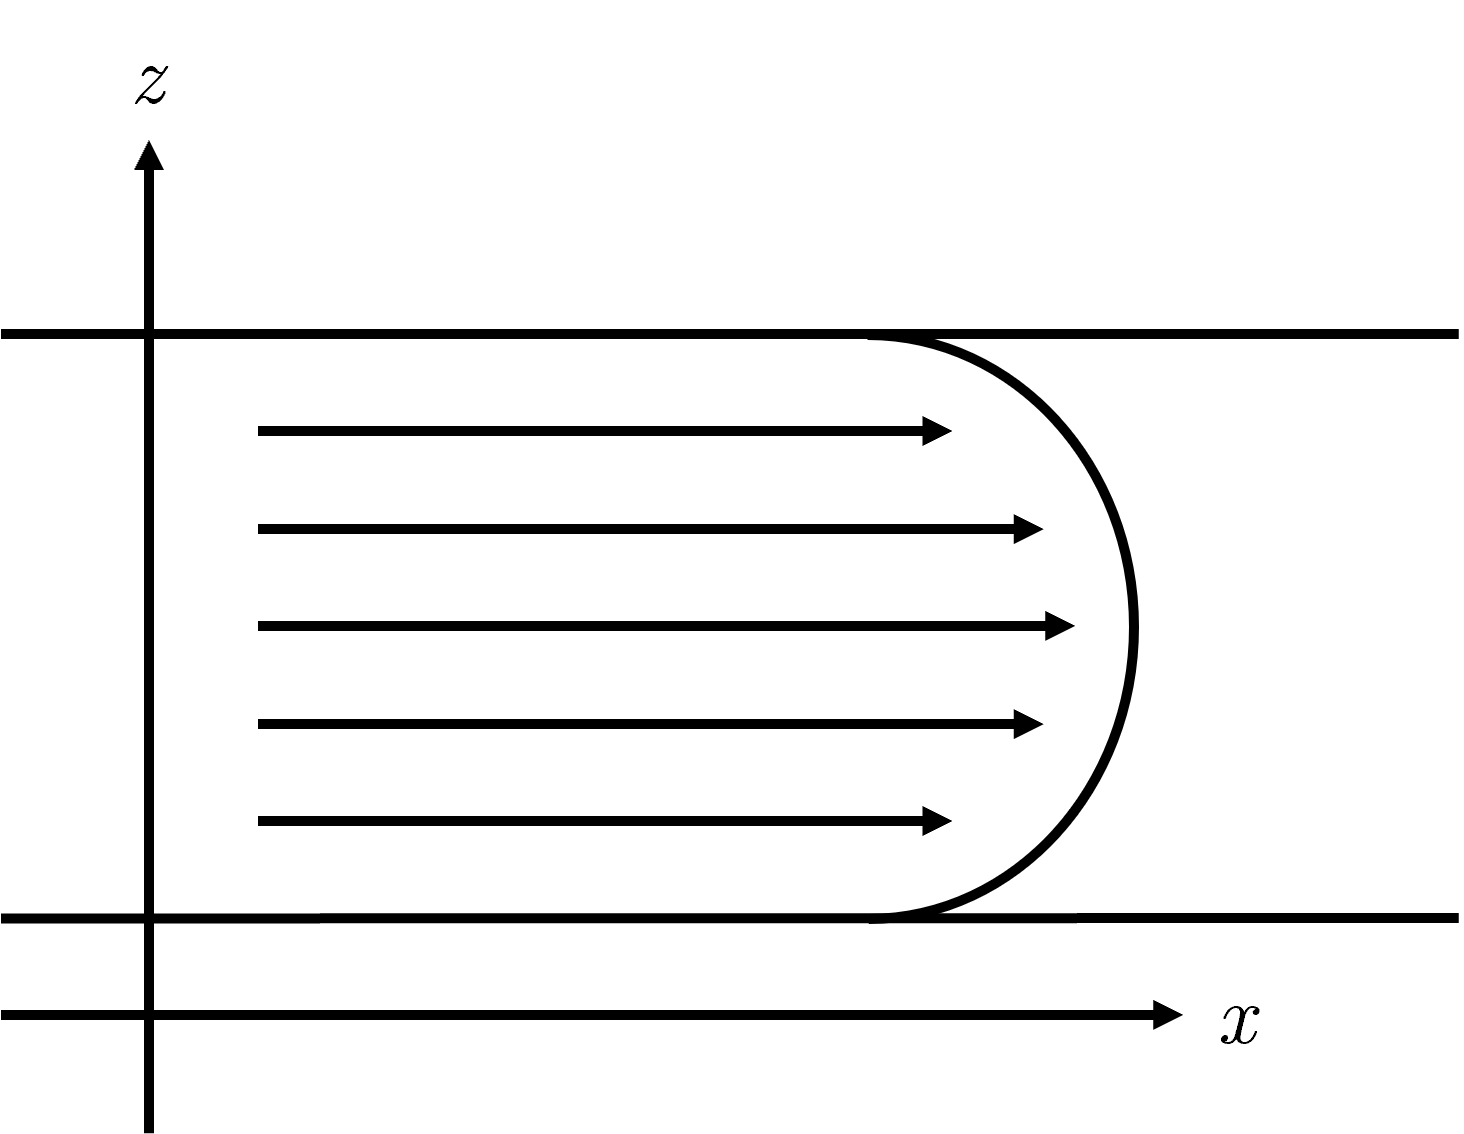
\includegraphics[width=80mm]{figures/PoiseuilleFlow.png}
    }
    \subfloat[Couette flow]{
    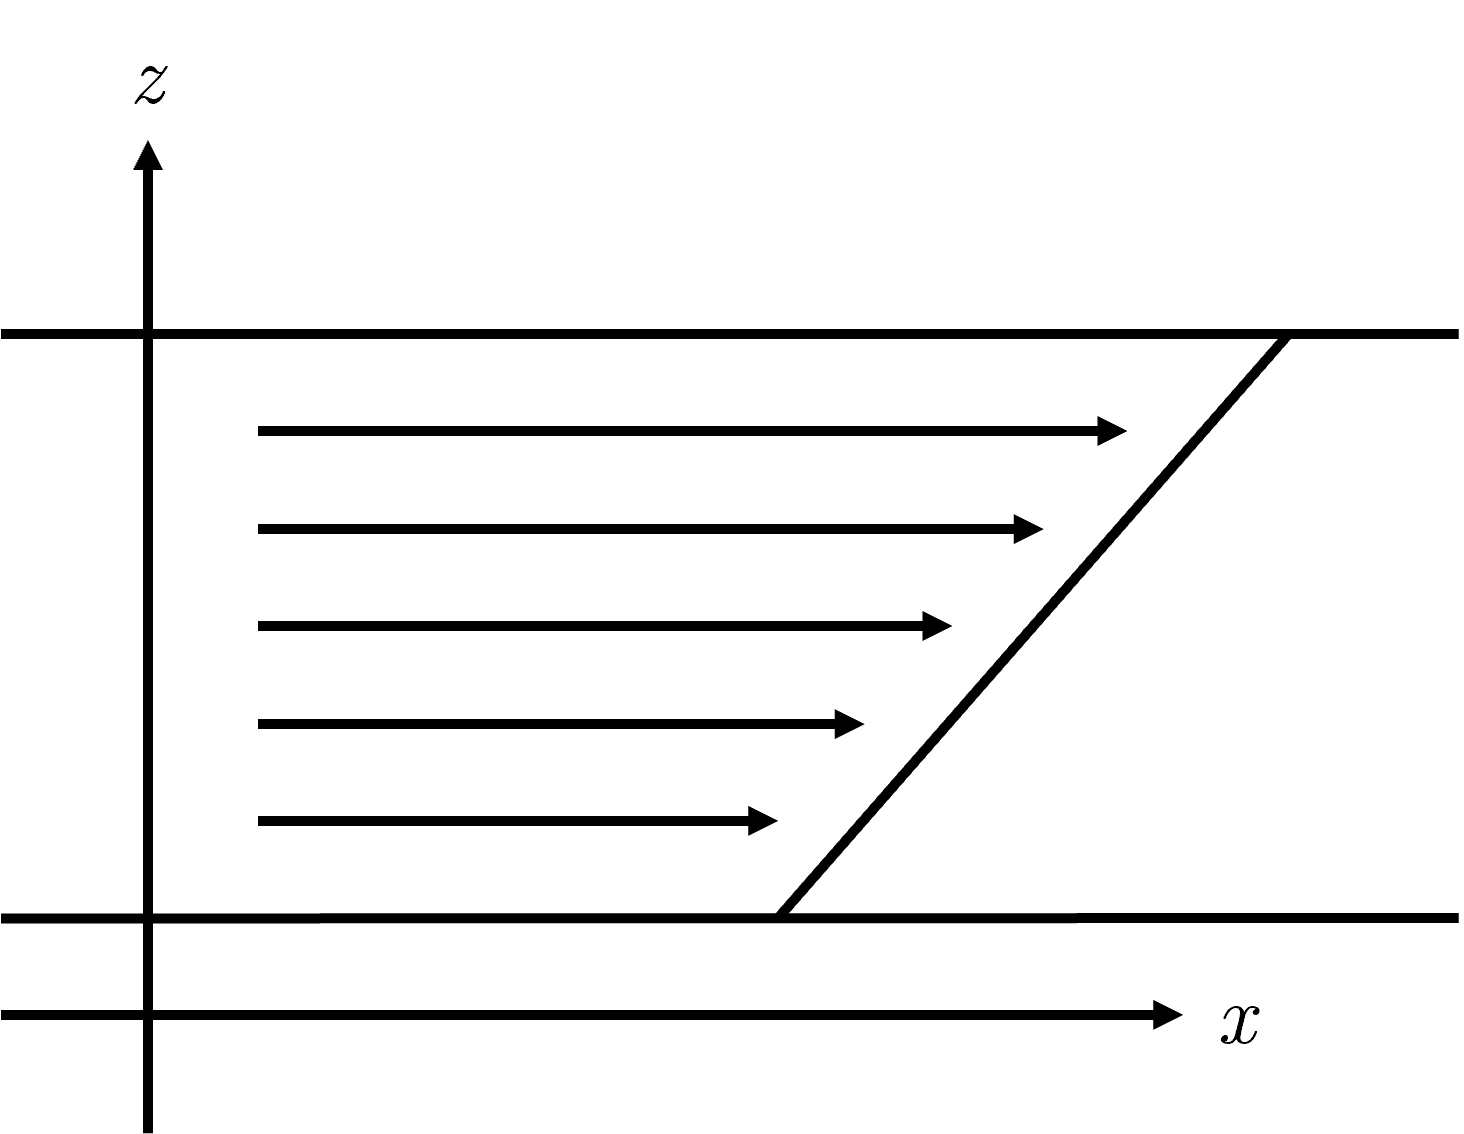
\includegraphics[width=80mm]{figures/CouetteFlow.png}
    }
    \caption{Schematics of plane Poiseuille and plane Couette flow}
    \label{fig:pandcflow}
\end{figure}




